\documentclass[compress]{beamer}
\usepackage{ifthen,verbatim}

\title{Proposed Track Filter for AlCaRecoMu}
\author{Jim Pivarski, Alexei Safonov}
\institute{Texas A\&M University}
\date{30 January, 2008}

\newcommand{\isnote}{}
\xdefinecolor{lightyellow}{rgb}{1.,1.,0.25}
\xdefinecolor{darkblue}{rgb}{0.1,0.1,0.7}

%% Uncomment this to get annotations
%% \def\notes{\addtocounter{page}{-1}
%%            \renewcommand{\isnote}{*}
%% 	   \beamertemplateshadingbackground{lightyellow}{white}
%%            \begin{frame}
%%            \frametitle{Notes for the previous page (page \insertpagenumber)}
%%            \itemize}
%% \def\endnotes{\enditemize
%% 	      \end{frame}
%%               \beamertemplateshadingbackground{white}{white}
%%               \renewcommand{\isnote}{}}

%% Uncomment this to not get annotations
\def\notes{\comment}
\def\endnotes{\endcomment}

\setbeamertemplate{navigation symbols}{}
\setbeamertemplate{headline}{\includegraphics[height=1 cm]{../cmslogo} \hspace{0.1 cm} \includegraphics[height=1 cm]{../tamulogo} \hfill
\begin{minipage}{5.5 cm}
\vspace{-0.75 cm} \small
\begin{center}
\ifthenelse{\equal{\insertpagenumber}{1}}{}{\textcolor{blue}{\insertsection}}
\end{center}
\end{minipage} \hfill
\begin{minipage}{4.5 cm}
\vspace{-0.75 cm} \small
\begin{flushright}
\ifthenelse{\equal{\insertpagenumber}{1}}{}{Jim Pivarski \hspace{0.5 cm} \insertpagenumber\isnote/\pageref{numpages}}
\end{flushright}
\end{minipage}\mbox{\hspace{0.2 cm}}}

\begin{document}
%% \frame{\titlepage}

\begin{notes}
\item This is the annotated version of my talk.
\item If you want the version that I am presenting, download the one
labeled ``slides'' on Indico (or just ignore these yellow pages).
\item The annotated version is provided for extra detail and a written
record of comments that I intend to make orally.
\item Yellow notes refer to the content on the {\it previous} page.
\item All other slides are identical for the two versions.
\end{notes}

%% \section*{How the track cut is defined}

%% \begin{frame}
%% \begin{columns}
%% \column{0.4\linewidth}
%% 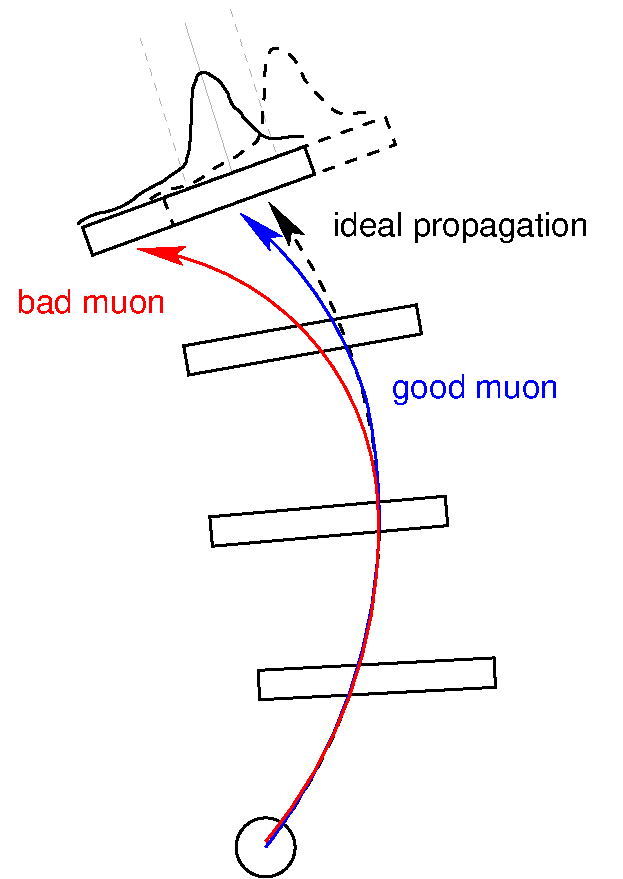
\includegraphics[width=1.1\linewidth]{trackcut.pdf}

%% \column{0.65\linewidth}
%% \textcolor{darkblue}{Loop over subsample:}
%% \begin{enumerate}
%% \item Use Propagator to extrapolate from reco::Muon's tracker track to
%% outermost muon station (MB4, ME1/3, ME3/2, ME4/1)

%% \item Fill ``propagated minus hit'' histograms for each chamber

%% \item Define window to be mean $\pm n$ stdev (e.g.\ $n=3$)
%% \end{enumerate}

%% \textcolor{darkblue}{Loop over whole dataset:}
%% \begin{enumerate}
%% \item Use Propagator to extrapolate from reco::Muon's tracker track to
%% outermost muon station

%% \item If ``propagated minus hit'' is within window, keep the track
%% \end{enumerate}
%% \end{columns}
%% \end{frame}

%% \begin{frame}
%% \begin{columns}
%% \column{0.4\linewidth}
%% 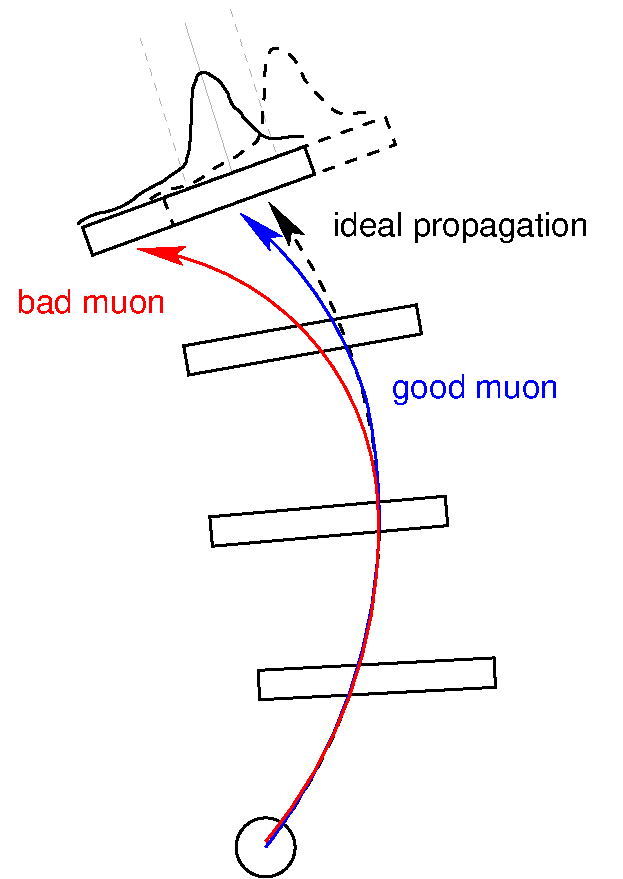
\includegraphics[width=1.1\linewidth]{trackcut.pdf}

%% \column{0.65\linewidth}
%% \textcolor{darkblue}{Features:}
%% \begin{itemize}
%% \item Cut criteria are independent of how the track is fitted in
%% alignment procedure
%% \begin{itemize}
%% \item By contrast, a cut on residuals depends strongly on the weight
%% of a muon hit in the fit (APE) and how much outside information is used
%% (globalMuon/standAlone/segment)
%% \end{itemize}

%% \item This is a cut on the consistency of the real muon (represented
%% by the hit) with the zero scattering hypothesis (represented by the
%% propagation)

%% \item Cut criteria are independent of the alignment of the outermost
%% muon station (that's why we need two loops: the first finds the chambers)
%% \end{itemize}
%% \end{columns}
%% \end{frame}

%% \begin{frame}
%% \begin{columns}
%% \column{0.4\linewidth}
%% 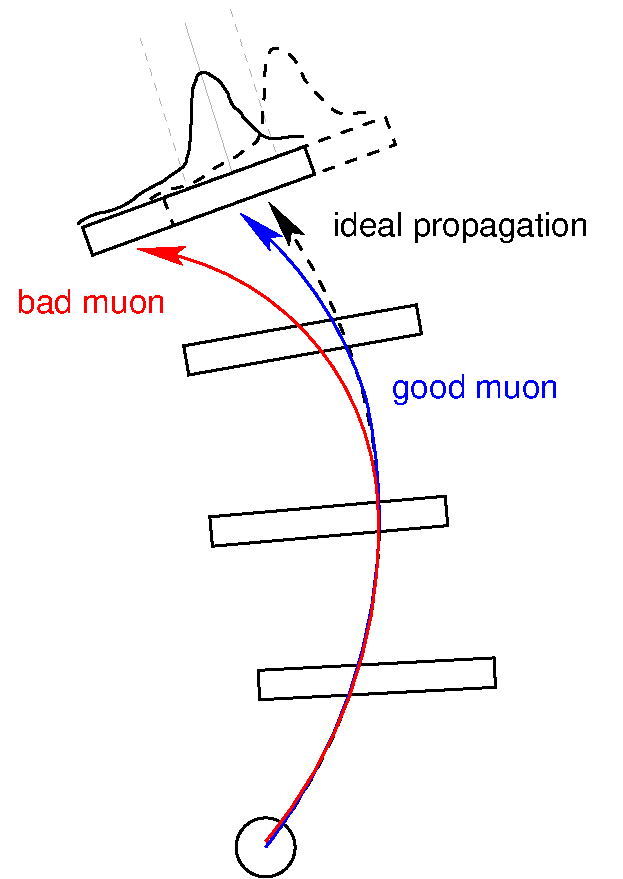
\includegraphics[width=1.1\linewidth]{trackcut.pdf}

%% \column{0.65\linewidth}
%% \textcolor{darkblue}{Disadvantages:}
%% \begin{itemize}
%% \item We need two loops (though the first one only needs to be long
%% enough to determine the mean and stdev of the residual distribution on
%% each chamber in MB4, ME1/3, ME3/2, and ME4/1)

%% \item Every muon needs to be propagated one more time (additional CPU
%% time $\le$ a full track fit)
%% \end{itemize}
%% \end{columns}
%% \end{frame}

%% \section*{Effect on alignment quality}

\begin{frame}
\begin{itemize}
\item Full 6-dof misalignment/realignment scenario
\item Simplified method for generic test:
\begin{enumerate}
\item align wheels/disks
\item align chambers with muon APE = $\infty$ globalMuons (100~pb$^{-1}$)
\end{enumerate}
\item Most improvement in MB2 and ME ring 2
\end{itemize}

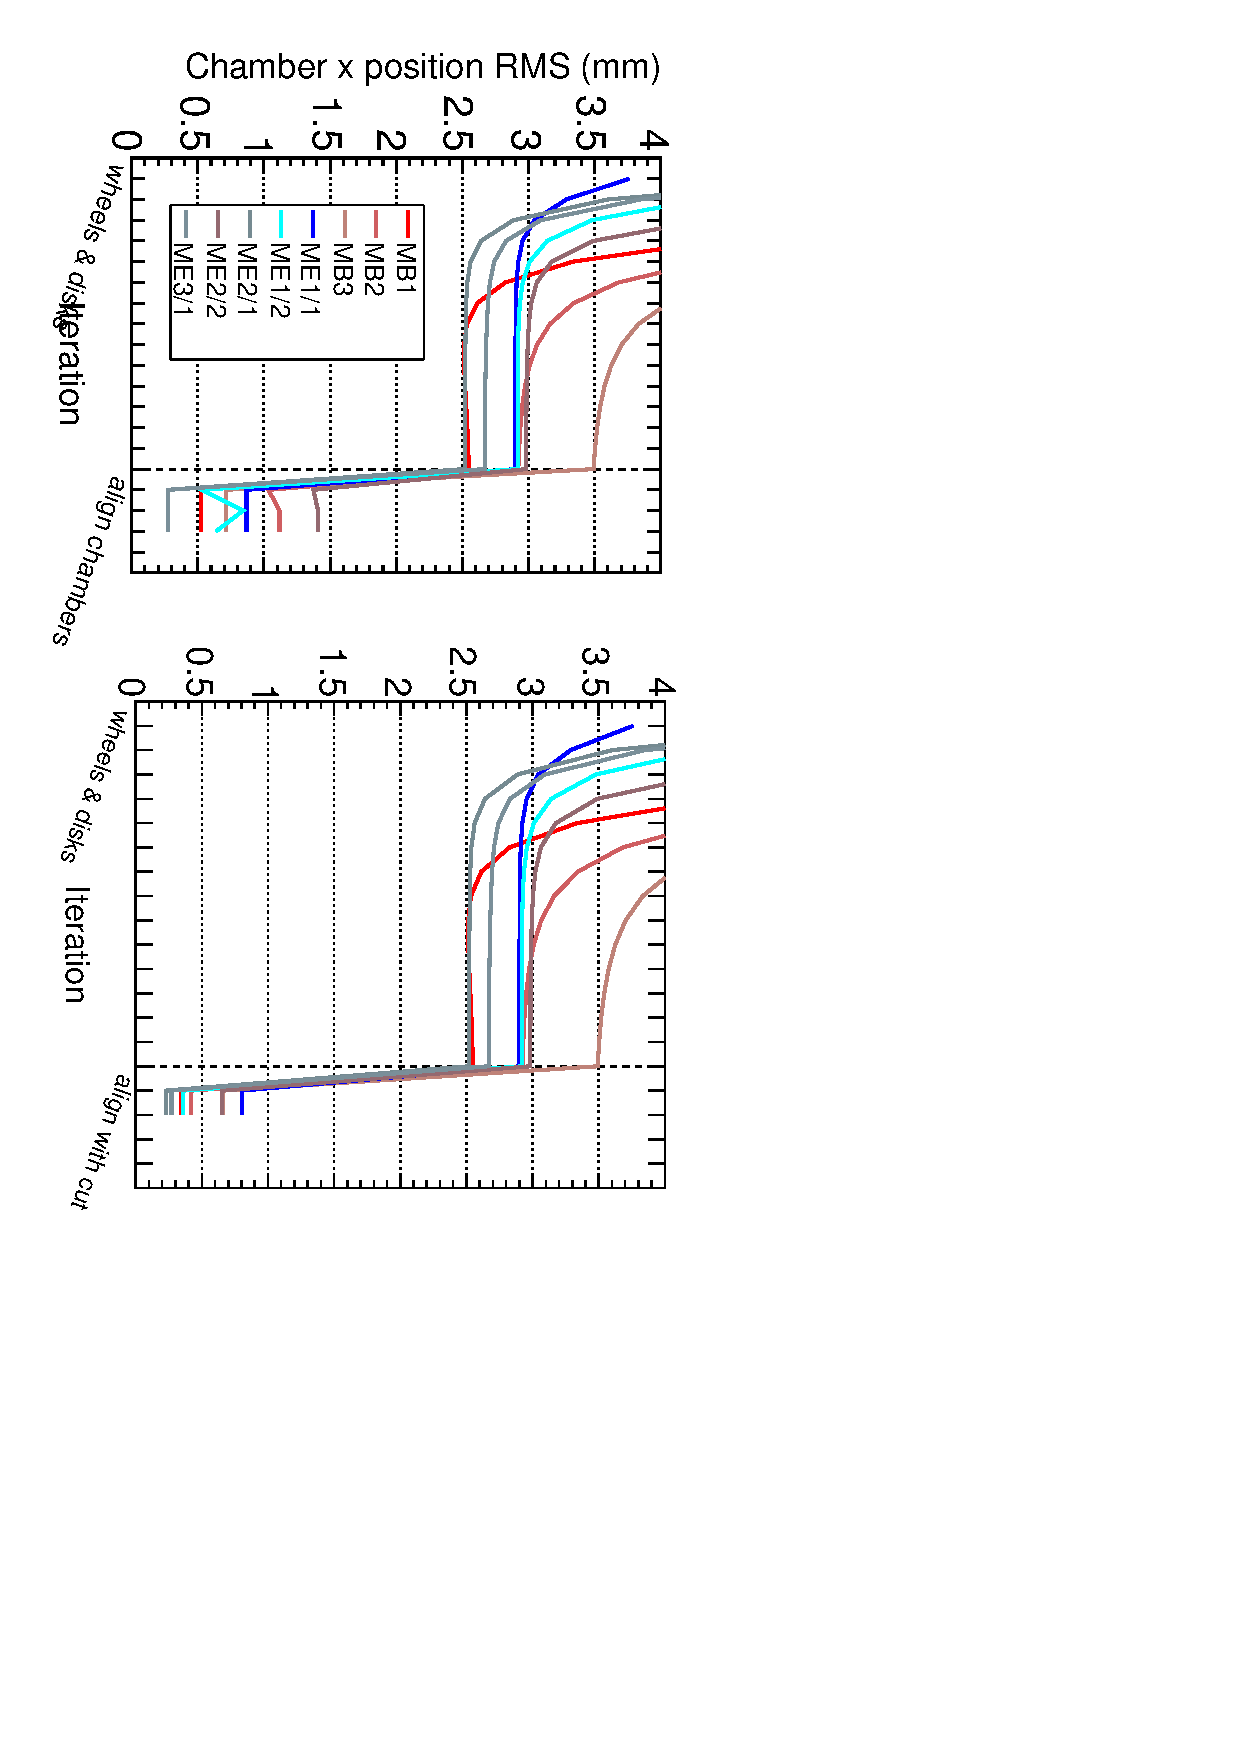
\includegraphics[height=\linewidth, angle=90]{compate_with_without_cut.pdf}
\end{frame}

%% \section*{Implementation Options}

\begin{frame}
\textcolor{darkblue}{Option \#1: special filters used only by HIP method}
\begin{itemize}
\item AlCaRecoMu and AlignmentMuonSelectorModule unaffected
\item We make a private, filtered copy of AlCaRecoMu stream (nearly
the same size as full stream)
\end{itemize}

\vfill
\textcolor{darkblue}{Option \#2: define cut in AlignmentMuonSelectorModule, but don't use it for official AlCaRecoMu}
\begin{itemize}
\item We make a private, filtered copy of AlCaRecoMu stream using
AlignmentMuonSelectorModule with the cut turned on
\item Safe: easy to verify {\tt applyScatteringFilter = false}
\end{itemize}

\vfill
\textcolor{darkblue}{Option \#3: apply the cut to AlCaRecoMu for both methods}
\begin{itemize}
\item Requires careful testing, because it's irreversible
\item Doesn't significantly impact quantity of data for high momentum ($p_T$ $>$ 20~GeV)
\item Possible to implement two event loops in Express Stream?
\item Don't need to decide between \textcolor{darkblue}{\#2} and \textcolor{darkblue}{\#3} for CMSSW\_2\_0\_0
\end{itemize}
\end{frame}

%% \section*{}

%% \begin{frame}
%% \frametitle{Conclusions}
%% \begin{itemize}\setlength{\itemsep}{0.5 cm}
%% \item We do not claim that the cut is fully tested (it should be
%% applied to MB4, ME1/3, ME3/2, ME4/1, and in our baseline ``one station
%% at a time'' procedure)

%% \item These are early indications that it can be very helpful (factors
%% of 2 and 3, depending on station)

%% \item We want to present it now, so it won't be a surprise later
%% \end{itemize}

%% \label{numpages}
%% \end{frame}

\end{document}
